\documentclass[11pt,a4paper]{article}

\usepackage[utf8]{inputenc}
\usepackage[T1]{fontenc}
\usepackage[spanish]{babel}
\usepackage[margin=2.5cm]{geometry}
\usepackage{lmodern}
\usepackage{array}
\usepackage{longtable}
\usepackage{graphicx}
\usepackage{fancyhdr}

\setlength{\parindent}{0pt}
\setlength{\parskip}{6pt}
\setlength{\headheight}{14pt}
\renewcommand{\arraystretch}{1.35}

\pagestyle{fancy}
\fancyhf{} 
\fancyfoot[C]{\thepage}
 

\begin{document} 

Nombre: Angelo Maximiliano Espinoza Pivaque

\section*{T1a}

Un requisito es la necesidad que se necesita cubrir, debe ser
coherente, medible, verificable y consistente

\section*{T1b}

StRS: Son los requisito que se deben cumplir por parte de los
interesados en este casos la director distrital, coordinadora de
inmunizaciones, responsables de vacunatorio, tecnico y los proveedores

SyRS: Son los requisitos que el sistema debe cumplir

SRS: Son los requisitos que el software debe cumplir

\begin{longtable}{|p{1cm}|p{1.6cm}|p{11.3cm}|}
\hline
ID & & \\
\hline
E1 & StRS &
Porqué es una especificación para la coordinadora de inmunizaciones \\
\hline
E2 & SyRS &
Porque el sistema debe conservar entre $+2\,^\circ$C y $+8\,^\circ$C \\
\hline
E3 & SyRS &
Porque El sensor es parte del sistema \\
\hline
E4 & SyRS &
Porque es una función que realiza el sistema \\
\hline
E5 & SyRS &
Es una función que realiza el sistema \\
\hline
E6 & SyRS &
Es una función que realiza el sistema \\
\hline
E7 & StRS &
Es una función que realiza los interesados \\
\hline
E8 & SRS &
Es una función que realiza el software \\
\hline
E9 & SySR &
Porque habla de instalar y eso es parte del sistema \\
\hline
E10 & StRS &
Es una función que realiza los interesado \\
\hline
E11 & SRS &
por que estamos hablando de como debe ser el software \\
\hline
E12 & StRS &
Es una función que la realizan los interesados \\
\hline
\end{longtable}

\newpage

\section*{T1c}

\begin{tabular}{|p{1cm}|p{5cm}|p{4cm}|}
\hline
ID & & \\
\hline
H1 & Elicitación & Central \\
\hline
H2 & Negociación & Central \\
\hline
H3 & Especificación & Central \\
\hline
H4 & Validación & transversal \\
\hline
H5 & Gestión & transversal \\
\hline
\end{tabular}

\section*{T2a}

\begin{longtable}{|p{0.8cm}|p{2.5cm}|p{1.9cm}|p{8.3cm}|}
\hline
ID & Tipo & Documento & Justificación \\
\hline
E1 & Funcional & StRS &
Porque nos habla de que debe hacer y para quien \\
\hline
E2 & Funcional & SySR &
Porque nos dice de que debe hacer el sistema \\
\hline
E3 & No Funcional & SySR &
No funcional de rendimiento porque envia lectura cada 20 min \\
\hline
E4 & proceso & SySR &
De proceso porque los desarrolladores deben cumplir \\
\hline
E5 & Funcional & SySR &
Funcional porque es la Acción que debe cumplir el sistema \\
\hline
E6 & Funcional & SyS1 &
Funcional porque es una acción del sistema \\
\hline
E7 & Dominio & StSR &
Dominio porque es una regla de negocio \\
\hline
E8 & No funcional rendimiento & SRS &
No funcional de rendimiento porque dice como debe funcionar \\
\hline
E9 & Restricción & SySR &
Porque limita a donde se instala la plataforma \\
\hline
E10 & funcional & StSR &
como funciona el sistema \\
\hline
E11 & No funcional & SRS &
Como debe funcionar la plataforma \\
\hline
E12 & Proceso & StSR &
Porque es parte de la entrevista \\
\hline
\end{longtable}

\clearpage

\section*{Anexo: fotografías de las hojas}

\subsection*{Hoja 1}

\begin{center}
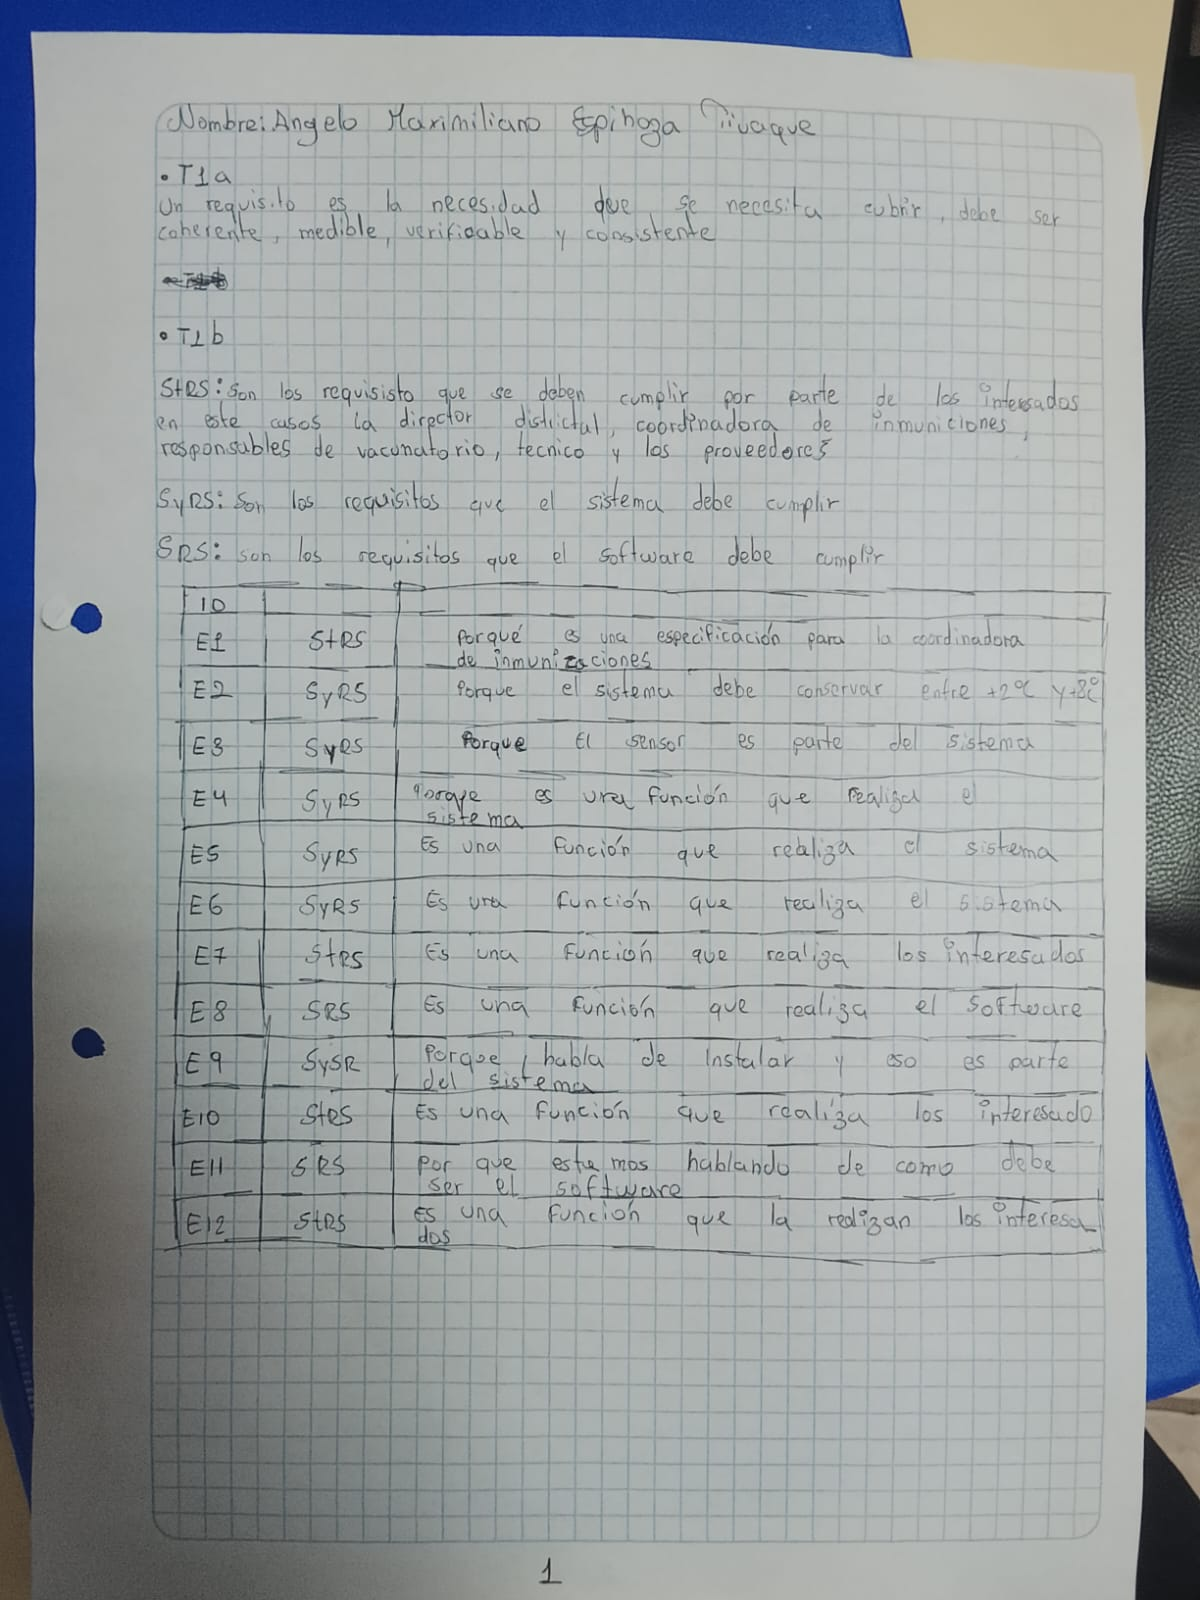
\includegraphics[
    width=\textwidth,
    height=0.82\textheight,
    keepaspectratio
]{evidencias/hoja-01.jpeg}
\end{center}

\clearpage

\subsection*{Hoja 2}

\begin{center}
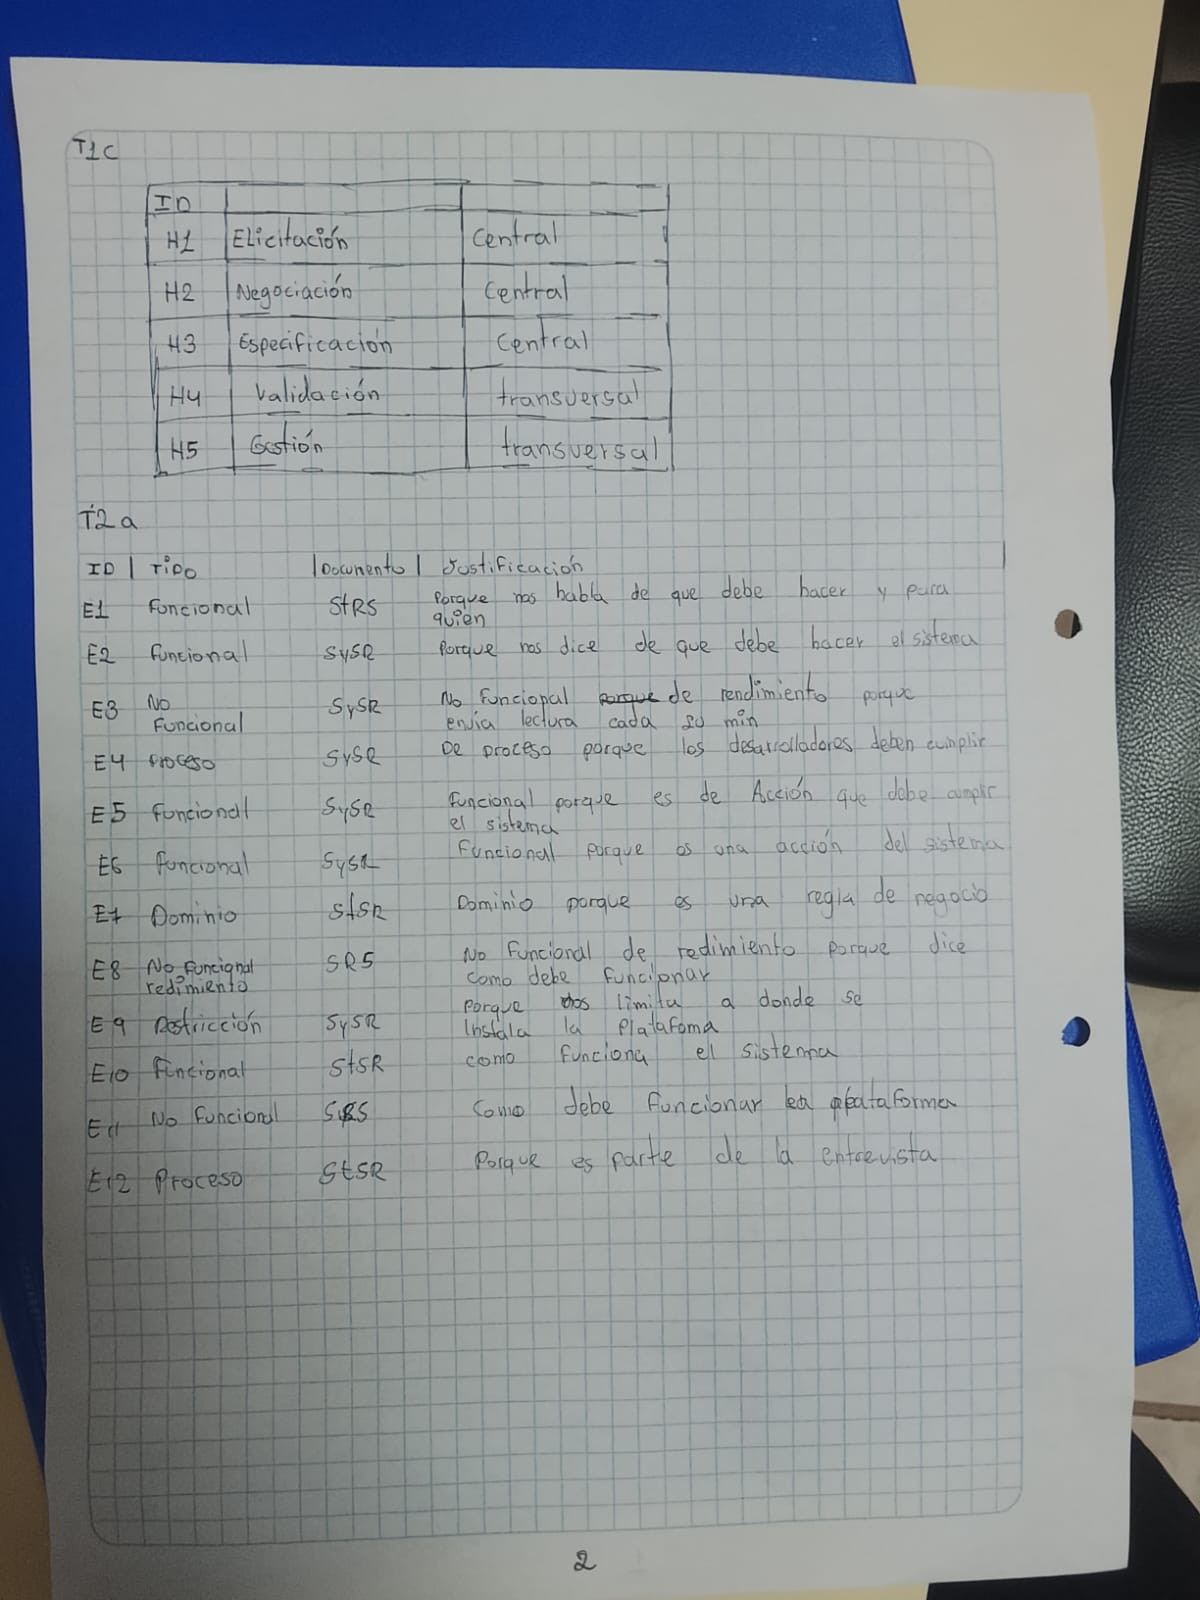
\includegraphics[
    width=\textwidth,
    height=0.85\textheight,
    keepaspectratio
]{evidencias/hoja-02.jpeg}
\end{center}

\end{document}